\documentclass[amsmath,secnumarabic,floatfix,amssymb,nofootinbib,nobibnotes,letterpaper,11pt,tightenlines,showkeys]{revtex4}

\usepackage{times}

\usepackage{geometry}
\usepackage{amssymb}
\usepackage{latexsym, amsmath, amscd,amsthm}
\usepackage{graphicx}
\usepackage{array}
\usepackage[percent]{overpic}
%\usepackage{pdfsync}
\usepackage{units}
\usepackage{hyperref}
\PassOptionsToPackage{caption=false}{subfig}
\usepackage[lofdepth]{subfig}

\usepackage{clrscode}

\def\figdir{figs/}
\graphicspath{\figdir}

\newtheorem{theorem}{Theorem}
\newtheorem*{maintheorem}{Main Theorem}
\newtheorem{lemma}[theorem]{Lemma}
\newtheorem{proposition}[theorem]{Proposition}
\newtheorem{corollary}[theorem]{Corollary}

\theoremstyle{definition}
\newtheorem{definition}[theorem]{Definition}
\newtheorem*{example}{Example}
\newtheorem{conjecture}[theorem]{Conjecture}
\newtheorem{remark}[theorem]{Remark}

\def\defn#1{Definition~\ref{def:#1}}
\def\thm#1{Theorem~\ref{thm:#1}}
\def\lem#1{Lemma~\ref{lem:#1}}
\def\figr#1{Figure~\ref{fig:#1}}
\def\prop#1{Proposition~\ref{prop:#1}}
\def\cor#1{Corollary~\ref{cor:#1}}
\def\sect#1{Section~\ref{sect:#1}}
\def\mainthm#1{Main Theorem~\ref{mainthm:#1}}
\def\mainthm#1{Main Theorem~\ref{mainthm:#1}}
\def\rmark#1{Remark~\ref{rmark:#1}}
%\numberwithin{equation}{section}

% make a small change

\newcommand{\abs}[1]{\lvert#1\rvert}
\newcommand{\tvnorm}[1]{\left| #1 \right|_{\operatorname{TV}}}
\newcommand{\R}{\mathbb{R}}
\newcommand{\C}{\mathbb{C}}
\newcommand{\Q}{\mathbb{H}}
\newcommand{\Z}{\mathbb{Z}}
\newcommand{\F}{\mathbb{F}}

\newcommand{\arc}[1]{\gamma_{#1}}
\newcommand{\len}[1]{\ell_{#1}}
\newcommand{\bdry}{\partial}
\newcommand{\bdy}{\bdry}
\newcommand{\isom}{\cong}
\newcommand{\setm}{\smallsetminus}
\newcommand{\eps}{\varepsilon}
\newcommand{\lk}{\textrm{lk}}
\newcommand{\intr}{\textrm{int}} %interior
\newcommand{\half}{\tfrac12}
\newcommand{\arcsec}{\textrm{arcsec}}
\newcommand{\m}{\mathcal}
\renewcommand{\d}{\partial}
\newcommand{\grad}{\nabla}
\newcommand{\PThree}{\ePol_3(n)/\SO(3)}
\newcommand{\EOne}{E_1}
\newcommand{\ETwo}{E_2}
\newcommand{\FOne}{F_1}

\newcommand{\loopinsert}{E_1}
\newcommand{\edgedouble}{E_2}
\newcommand{\cutedgedouble}{E_3}
\newcommand{\pairinsert}{E_4}
\newcommand{\plantri}{\texttt{plantri} }
\newcommand{\nauty}{\texttt{nauty} }
\newcommand{\saucy}{\texttt{saucy} }


\graphicspath{{../../figs/}{figs/}}

\newcommand{\eightgraph}{\raisebox{-0.17\baselineskip}{\includegraphics[height=0.81\baselineskip]{eightgraph}}}
\newcommand{\hopfgraph}{\raisebox{-0.17\baselineskip}{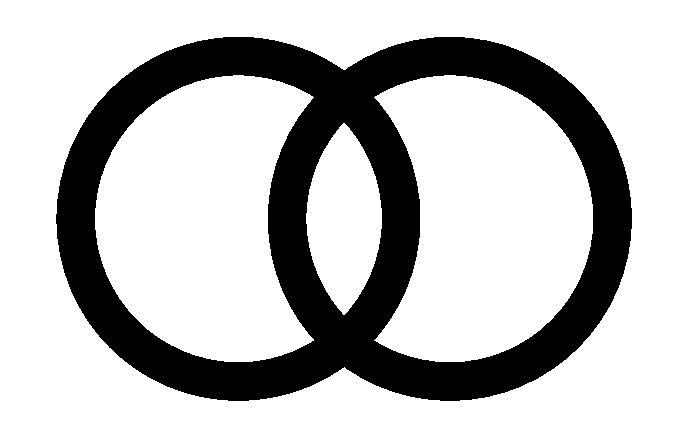
\includegraphics[height=0.81\baselineskip]{hopfgraph}}}


\bibliographystyle{plain}
%
\def\co{\colon\!}

\setlength{\parskip}{5pt}

\let\mgp=\marginpar \marginparwidth18mm \marginparsep1mm
\def\marginpar#1{\mgp{\raggedright\tiny #1}}
%\def\marginpar#1{}   %Uncomment this to hide all marginpars

\let\lbl=\label
\def\label#1{\lbl{#1}\ifinner\else\marginpar{\ref{#1} #1}\ignorespaces\fi}

\bibliographystyle{plain}

\begin{document}
\title[]{Isomorphisms of Multigraphs in Terms of Isomorphisms of Colored Simple Graphs}
\author{Jason Cantarella, Harrison Chapman, Eric Lybrand, Hollis Neel and Malik Henry}
\altaffiliation{University of Georgia, Mathematics Department, Athens GA}
\noaffiliation
\author{Matt Mastin}
\altaffiliation{Wake Forest University, Mathematics Department, Athens GA}
\noaffiliation
\author{Eric Rawdon(?)}
\altaffiliation{Wake Forest University, Mathematics Department, Athens GA}
\noaffiliation

\maketitle

\begin{definition}
	A \textbf{multigraph} $G$ is a triple $G = (V,E,f)$ where $V$ is a finite set of \emph{vertices}, $E$ is a finite set of \emph{edges}, and $f$ is a map from $E$ to the power set of $V$, $\m{P}(V)$, so that $f(e)$ is a subset of size either $1$ or $2$. The vertices in $f(e)$ are called the \textbf{endpoints} of $e$. Edges with $\abs{f(e)}=1$ are called \textbf{loops}.

An \textbf{isomorphism} from a graph $G_1$ to a graph $G_2$ is a pair of bijections $(\phi_V,\phi_E)$ with $\phi_V: V_1 \rightarrow V_2$ and $\phi_E: E_1 \rightarrow E_2$ such that $(\phi_V \circ f_1)(e)=(f_2 \circ \phi_E)(e)$ (as sets) for all $e \in E_1$.

A \textbf{coloring on the vertices} of a graph is a map, $C_V$, from $V$ to a set of colors $X$. An isomorphism $(\phi_V, \phi_E)$ from a vertex colored graph $G_1$ to a vertex colored graph $G_2$ \textbf{respects the vertex coloring} if, and only if, $C_{V_1}(v) = (C_{V_2} \circ \phi_V)(v)$ for all $v \in V_1$. 

A \textbf{coloring on the edges} of a graph is a map, $C_E$, from $E$ to a set of colors $X$. An isomorphism $(\phi_V, \phi_E)$ from an edge colored graph $G_1$ to an edge colored graph $G_2$ \textbf{respects the edge coloring} if, and only if, $C_{E_1}(e) = (C_{E_2} \circ \phi_E)(e)$ for all $e \in E_1$. 

%An isomorphism $\phi$ from a colored graph $G_1$ to a colored graph $G_2$ \textbf{respects the edge coloring} if $\phi^{-1} \circ C_{E_1} = C_{E_2} \circ \phi$. 


\end{definition}



\begin{definition}{\label{gbar}}
	Given a multigraph $G=(V,E,f)$ we define an associated graph $\bar{G} = (\bar{V}, \bar{E}, \bar{f})$ by the following construction. 

	\begin{itemize}
		\item The vertices of $\bar{G}$ are the vertices of $G$, in other words, $\bar{V} = V$.
		\item The edges of $\bar{G}$ come from collapsing non-loop edges that have the same endpoints. We do this by defining the edges of $\bar{G}$ to be a set of preimages of $f$. In particular, set $$\bar{E} =  \{f^{-1}(f(v)) : \abs{f(v)} = 2\}.$$
		\item $\bar{f}(\bar{e}) = f(e)$ where $e$ is any element of $\bar{e}$. Note that this is well-defined as all edges in the set $\bar{f}(\bar{e})$ have the same endpoints by construction.
		
	\end{itemize}

	We also define a coloring on the vertices and edges of $\bar{G}$ as follows.
	
	\begin{itemize}
		\item $C_{\bar{V}}(\bar{v}) = $ the number of edges $e \in E$ such that $f(e) = \{v\}$.
		\item $C_{\bar{E}}(\bar{e}) = \abs{\bar{e}}$.  %where $e$ is any element of $\bar{e}$.
	\end{itemize}

\end{definition}

\begin{lemma}
	Given any graph $G$ the associated graph $\bar{G}$ is simple.
\end{lemma}

\begin{proof}
	An edge in $G$ is a loop precisely when $\abs{f(v)} = 1$ which is excluded in the definition of $\bar{G}$. Similarly, duplicate edges are not allowed in $\bar{E}$ because it is defined to be the \emph{set} of pre-images. Thus, $\bar{G}$ has no loops or multiedges and is therefore simple.
\end{proof}

Since $\bar{G} = (\bar{V}, \bar{E}, \bar{f})$ is always simple it can be described by only its set of vertices $\bar{V}$ and a collection of two element subsets of $\bar{V}$ giving the edges. In this case, a bijection $\bar{\phi}_V: \bar{V}_1 \rightarrow \bar{V}_2$ induces a map on the edge sets by $\bar{\phi}_E(\bar{e}) = \{\bar{\phi}_V(\bar{v}),\bar{\phi}_V(\bar{w})\}$. Thus, an isomorphism between simple graphs can be described by only a bijection on the vertex sets.

%\begin{definition}
%	Given a \emph{simple} graph $\bar{G}$ we define an \textbf{edge coloring} on $\bar{G}$ to be a map $C_{\bar{E}}$ from the edges of $\bar{G}$ to a set of colors $X$. Since $\bar{G}$ is simple we may regard $C_{\bar{E}}$ as a map from the two element subsets of $\bar{V}$ to the set of colors $X$. An isomorphism $\phi$ from an edge colored simple graph $G_1$ to an edge colored simple graph $G_2$ \textbf{respects the edge coloring} if $\phi^{-1} \circ C_{\bar{E}_1} = C_{\bar{E}_2} \circ \phi$. 
%\end{definition}

%\begin{definition}{\label{color}}
%	Given a multigraph $G=(V,E,f)$ we define a vertex coloring and an edge coloring on the associated graph $\bar{G}$ as follows.
%	
%	\begin{itemize}
%		\item $C_{\bar{V}}(\bar{v}) = $ the number of edges $e \in E$ such that $f(e) = \{v\}$.
%		\item $C_{\bar{E}}(\bar{e}) = f(e)$ where $e$ is any element of $\bar{e}$.
%	\end{itemize}
%
%	Note that $C_{\bar{E}}$ is well-defined since, by construction, all edges $e \in \bar{e}$ have the same endpoints.
%\end{definition}

\begin{theorem}
	Let $G_1$ and $G_2$ be multigraphs and $\bar{G}_1$ and $\bar{G}_2$ the associated colored graphs given in Definition \ref{gbar}. Then, given an isomorphism $\bar{\phi}$ from $\bar{G}_1$ to $\bar{G}_2$ that respects the vertex and edge coloring, we can construct a set of isomorphisms $\Phi(\bar{\phi}) = \{(\phi^1_V,\phi^1_E),\ldots,(\phi^k_V,\phi^k_E)\}$ from $G_1$ to $G_2$. In addition, $\Phi(\bar{\phi}_1)$ and $\Phi(\bar{\phi}_2) $ are disjoint if, and only if, $\bar{\phi}_1$ and $\bar{\phi}_2$ are distinct isomorphisms. Moreover, if $(\phi_V,\phi_E)$ is an isomorphism from $G_1$ to $G_2$, then there exists an isomorphism $\bar{\phi}$ from $\bar{G}_1$ to $\bar{G}_2$ such that $(\phi_V,\phi_E)$ will be produced by this construction. 
\end{theorem}

\begin{proof}
	We will first describe the construction and then prove that it satisfies the properties in the theorem.

	IDEA: $\phi^i_V = \bar{\phi}$ for all $i$ and each $\phi^i_E$ comes from all choices of permutations of the elements of each \emph{set} labeling each edge of $\bar{G}$.
\end{proof}

\bibliography{knotprobabilitypapers}


\end{document}
